% Fig. 3: (a) schematic diagram of the apparatus setup, (b) flow chart of data logging and analysis.
% Lynx settings from photographs of its settings pages, 27 October 2026. File formats and channel widths from results/interim/ir_file_formats.csv.
\documentclass[11pt,border=4pt]{standalone}
\usepackage[T1]{fontenc}
\usepackage{newtxtext}
\usepackage{amsmath}
\usepackage{newtxmath}
\usepackage{xcolor}
\usepackage{siunitx}
\usepackage{tikz}
\usetikzlibrary{arrows.meta,positioning,calc}
\newcommand{\nuc}[2]{\textsuperscript{#1}#2}
\newcommand{\seetag}[1]{\par\vspace{2pt}\hfill{\setlength{\fboxsep}{1.5pt}\fcolorbox{blue!45!black}{white}{\textcolor{blue!45!black}{see #1}}}}
\begin{document}
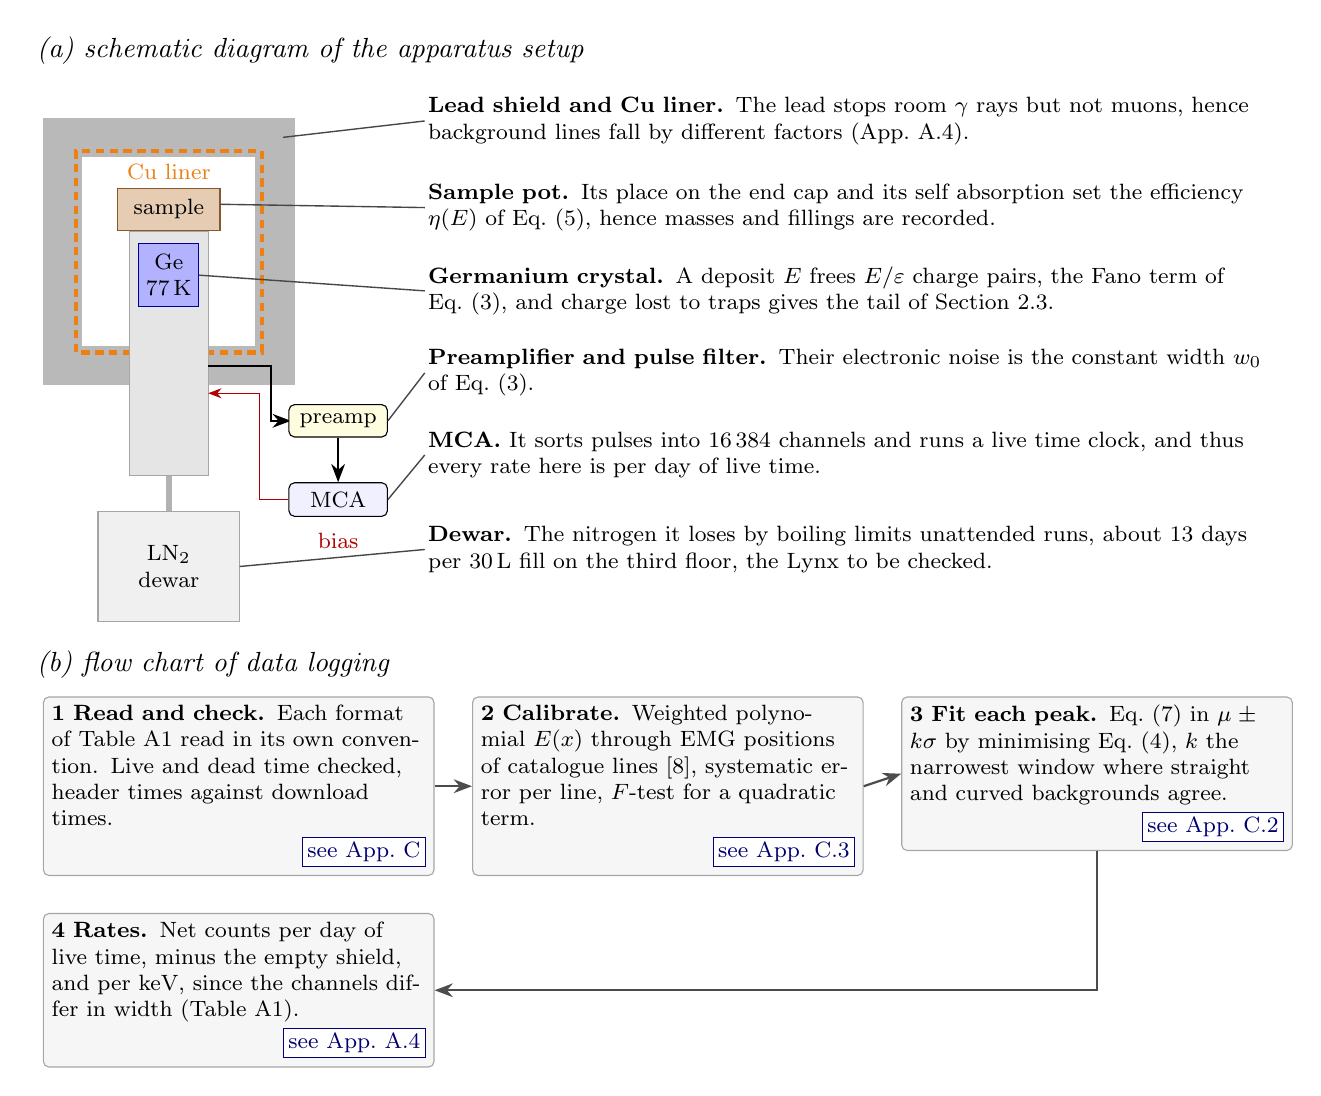
\begin{tikzpicture}[font=\footnotesize, >=Stealth,
  part/.style={anchor=north west, align=left, text width=10.9cm, inner sep=1pt},
  lead/.style={gray!55!black, line width=0.5pt},
  chainbox/.style={draw=gray!70, rounded corners=2pt, fill=gray!7, align=left, text width=4.75cm, minimum height=1.95cm,
               anchor=north west, inner sep=3pt}]
% ---------------------------------------------------------------- (a) the apparatus
\node[anchor=west, font=\normalsize\itshape] at (-0.2,4.25) {(a) schematic diagram of the apparatus setup};
\fill[gray!55] (0,0) rectangle (3.2,3.4);
\draw[orange!70!brown, line width=1.6pt, dash pattern=on 3pt off 2pt] (0.42,0.42) rectangle (2.78,2.98);
\fill[white] (0.5,0.5) rectangle (2.7,2.9);
\node[orange!70!brown] at (1.6,2.71) {Cu liner};
\fill[gray!20, draw=gray!70] (1.1,-1.15) rectangle (2.1,1.95);
\fill[blue!30, draw=blue!60!black] (1.22,1.0) rectangle (1.98,1.8);
\fill[brown!40, draw=brown!70!black] (0.95,1.97) rectangle (2.25,2.5);
\node at (1.6,2.235) {sample};
\node[align=center] at (1.6,1.4) {Ge\\77\,K};
\draw[line width=2pt, gray!60] (1.6,-1.15) -- (1.6,-1.6);
\fill[gray!12, draw=gray!70] (0.7,-3.0) rectangle (2.5,-1.6);
\node[align=center] at (1.6,-2.3) {LN$_2$\\dewar};
\draw[->, thick] (2.1,0.25) -- (2.9,0.25) |- (3.15,-0.45);
\node[draw, rounded corners=2pt, fill=yellow!12, minimum width=1.25cm] (pre) at (3.75,-0.45) {preamp};
\node[draw, rounded corners=2pt, fill=blue!6, minimum width=1.25cm] (mca) at (3.75,-1.45) {MCA};
\draw[->, thick] (pre) -- (mca);
\draw[->, red!70!black] (mca.west) -| (2.75,-0.1) -- (2.1,-0.1);
\node[red!70!black, anchor=north] at (3.75,-1.75) {bias};
\def\cx{4.85}
\node[part] (t1) at (\cx,3.7) {\textbf{Lead shield and Cu liner.} The lead stops room $\gamma$ rays but not muons, hence background lines fall by different factors (App.~A.4).};
\node[part] (t2) at (\cx,2.6) {\textbf{Sample pot.} Its place on the end cap and its self absorption set the efficiency $\eta(E)$ of Eq.~(5), hence masses and fillings are recorded.};
\node[part] (t3) at (\cx,1.55) {\textbf{Germanium crystal.} A deposit $E$ frees $E/\varepsilon$ charge pairs, the Fano term of Eq.~(3), and charge lost to traps gives the tail of Section~2.3.};
\node[part] (t4) at (\cx,0.5) {\textbf{Preamplifier and pulse filter.} Their electronic noise is the constant width $w_0$ of Eq.~(3).};
\node[part] (t5) at (\cx,-0.55) {\textbf{MCA.} It sorts pulses into 16\,384 channels and runs a live time clock, and thus every rate here is per day of live time.};
\node[part] (t6) at (\cx,-1.75) {\textbf{Dewar.} The nitrogen it loses by boiling limits unattended runs, about 13 days per 30\,L fill on the third floor, the Lynx to be checked.};
\draw[lead] (t1.west) -- (3.05,3.15);
\draw[lead] (t2.west) -- (2.25,2.3);
\draw[lead] (t3.west) -- (1.98,1.4);
\draw[lead] (t4.west) -- (pre.east);
\draw[lead] (t5.west) -- (mca.east);
\draw[lead] (t6.west) -- (2.5,-2.3);
% ---------------------------------------------------------------- (b) the analysis chain
\node[anchor=west, font=\normalsize\itshape] at (-0.2,-3.55) {(b) flow chart of data logging};
\node[chainbox] (s1) at (0,-3.95) {\textbf{1 Read and check.} Each format of Table~A1 read in its own convention. Live and dead time checked, header times against download times.\seetag{App.~C}};
\node[chainbox] (s2) at (5.45,-3.95) {\textbf{2 Calibrate.} Weighted polynomial $E(x)$ through EMG positions of catalogue lines~[8], systematic error per line, $F$-test for a quadratic term.\seetag{App.~C.3}};
\node[chainbox] (s3) at (10.9,-3.95) {\textbf{3 Fit each peak.} Eq.~(7) in $\mu \pm k\sigma$ by minimising Eq.~(4), $k$ the narrowest window where straight and curved backgrounds agree.\seetag{App.~C.2}};
\node[chainbox] (s4) at (0,-6.7) {\textbf{4 Rates.} Net counts per day of live time, minus the empty shield, and per keV, since the channels differ in width (Table~A1).\seetag{App.~A.4}};
\draw[->, thick, gray!60!black] (s1.east) -- (s2.west);
\draw[->, thick, gray!60!black] (s2.east) -- (s3.west);
\draw[->, thick, gray!60!black] (s3.south) |- (s4.east);
% ---------------------------------------------------------------- (c) the two systems and (d) the six spectra
\end{tikzpicture}
\end{document}
